% This is part of Un soupçon de mathématique sans être agressif pour autant
% Copyright (c) 2015
%   Laurent Claessens
% See the file fdl-1.3.txt for copying conditions.

\begin{exercice}[\ldots\ldots/4\cite{NRHooXFvgpp5}]\label{exo2smath-0163}

Arnaud a placé ses deux équerres identiques sur la droite $(d)$ comme l'illustre le schéma ci-dessous :
\begin{center}
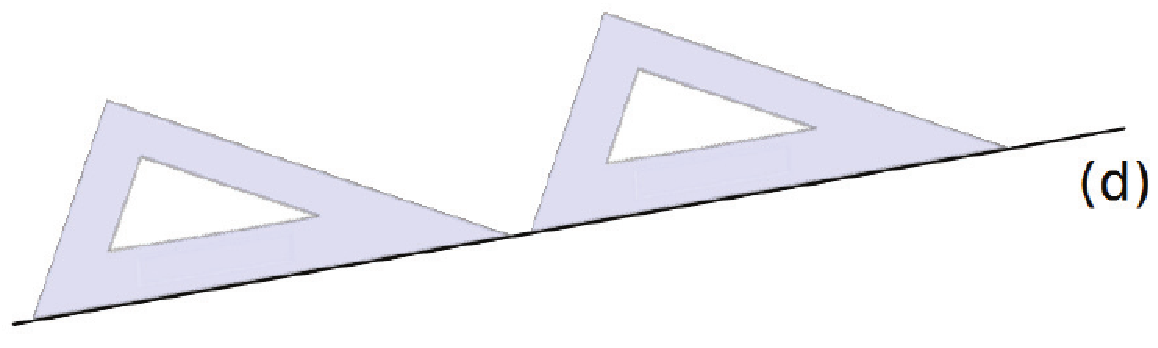
\includegraphics[width=7cm]{exoequerre.pdf}
\end{center}
Il affirme que, de cette façon, il peut tracer des droites parallèles. Est-ce vrai et pourquoi ?

\corrref{2smath-0163}
\end{exercice}
